    \begin{figure}[!htbp]
        \centering
        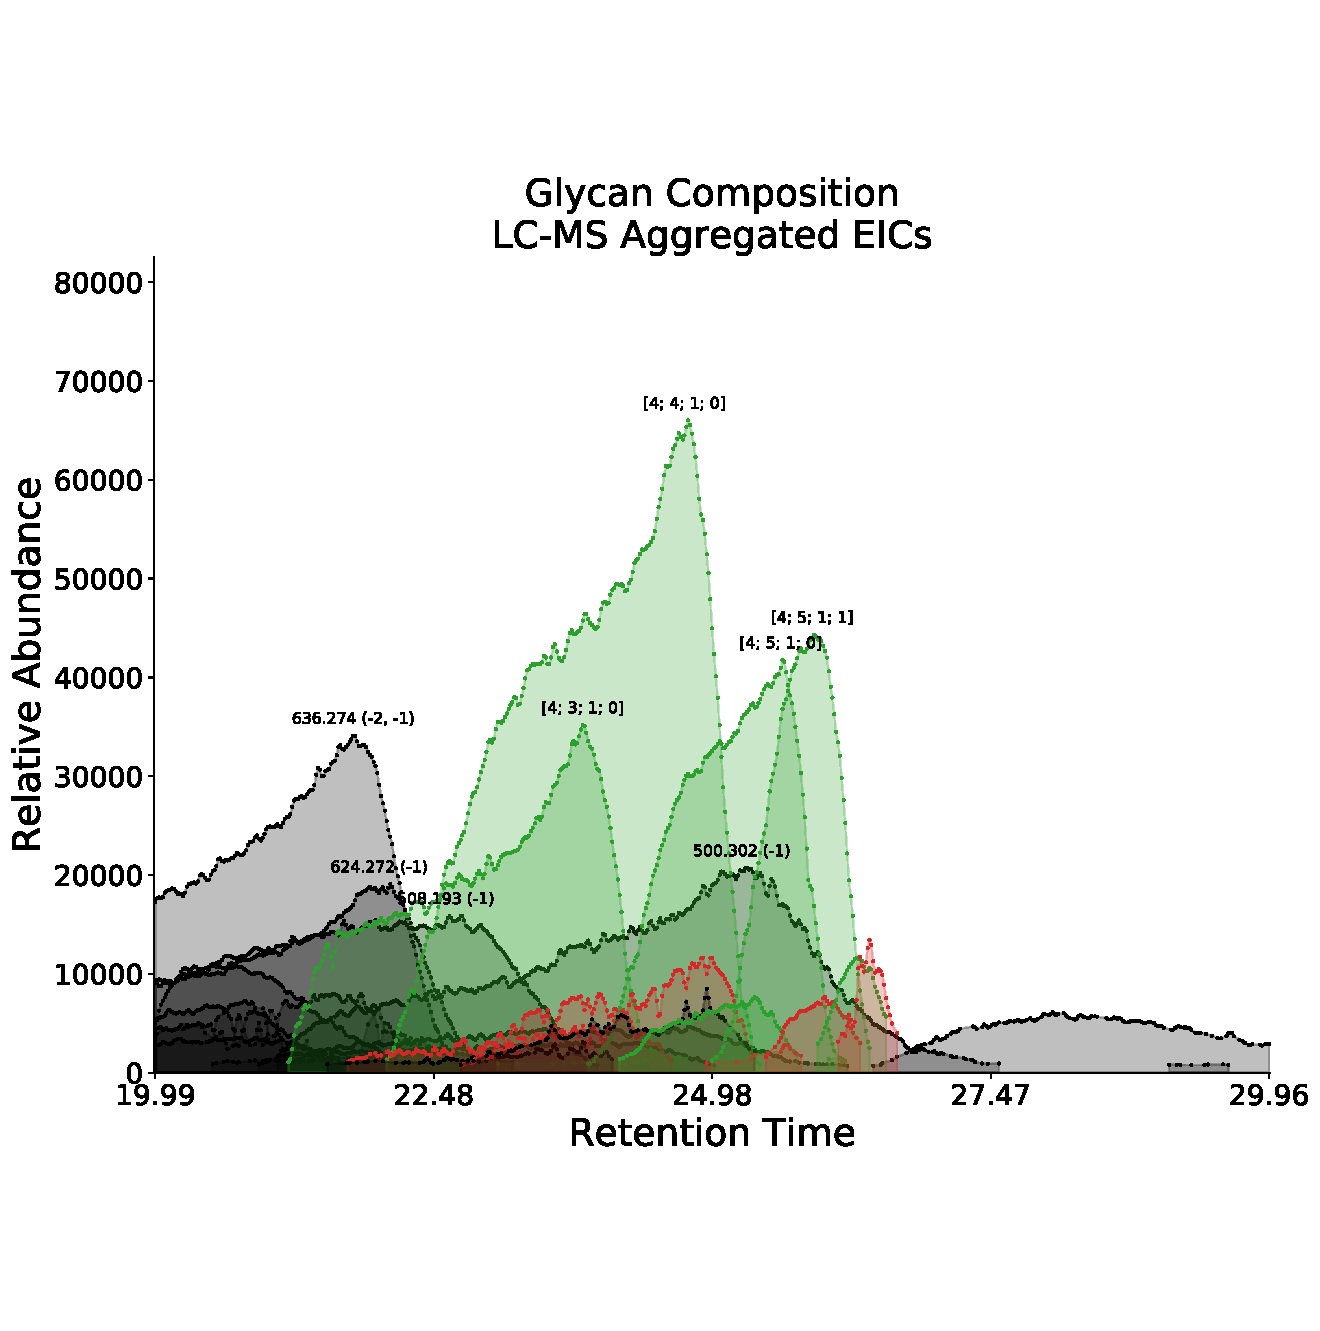
\includegraphics[width=0.45\textwidth,valign=t]{figure/igg_chromatograms.pdf}
        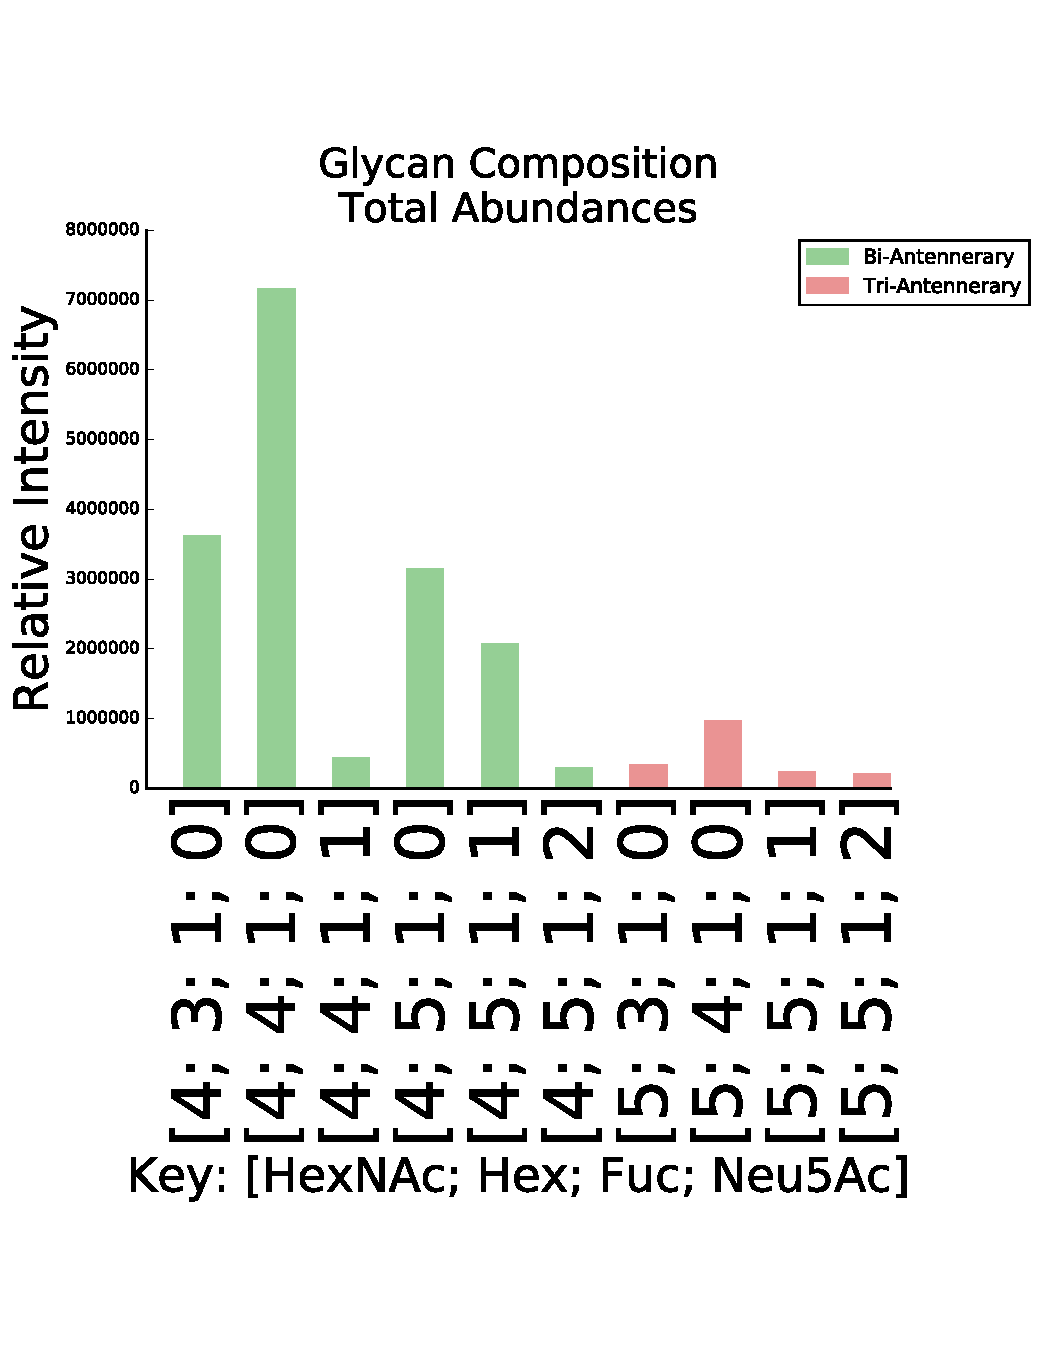
\includegraphics[width=0.45\textwidth,valign=t]{figure/igg_abundances.pdf}
        \caption{\textit{20151002-02-IGG} Glycan Relative Abundances}
        \label{fig:igg_aggregated_eics}
    \end{figure}

    \begin{table}
        \begin{minipage}[t]{0.25\linewidth}
            \vspace{0pt}
            (a)
            \centering
            
    \begin{tabular}{l | c}
        Group & $\tau$ \\
        \hline
        high-mannose & 0.00 \\
        hybrid & 14.58 \\
        bi-antennary & 8.67 \\
        asialo-bi-antennary & 14.47 \\
        tri-antennary & 5.30 \\
        asialo-tri-antennary & 11.61 \\
        tetra-antennary & 3.09 \\
        asialo-tetra-antennary & 0.00 \\
        penta-antennary & 0.00 \\
        asialo-penta-antennary & 0.00 \\
    \end{tabular}
    
            
        \end{minipage}
        \hspace{1cm}
        \begin{minipage}[t]{0.55\linewidth}
            \vspace{0pt}
            (b)
            \centering
            
    \begin{footnotesize}
    \begin{tabular}{l|p{2cm} p{2cm}}
Glycan Compostion &  Unregularized Score &  Regularized Score \\
\hline
\{Fuc:1; Hex:3; HexNAc:4\}           &                15.51 &              14.77 \\
\{Fuc:1; Hex:4; HexNAc:4\}           &                18.95 &              14.66 \\
\{Fuc:1; Hex:4; HexNAc:4; Neu5Ac:1\} &                13.23 &              12.23 \\
\{Fuc:1; Hex:5; HexNAc:4\}           &                18.23 &              14.52 \\
\{Fuc:1; Hex:5; HexNAc:4; Neu5Ac:1\} &                14.11 &              12.29 \\
\{Fuc:1; Hex:5; HexNAc:4; Neu5Ac:2\} &                11.78 &              10.95 \\
\{Fuc:1; Hex:3; HexNAc:5\}           &                11.41 &              14.15 \\
\{Fuc:1; Hex:4; HexNAc:5\}           &                15.34 &              13.57 \\
\{Fuc:1; Hex:5; HexNAc:5; Neu5Ac:1\} &                10.30 &               8.80 \\
\{Fuc:1; Hex:5; HexNAc:5; Neu5Ac:2\} &                14.07 &               7.54 \\
\end{tabular}

    \end{footnotesize}
    
        \end{minipage}
        \caption{
                 Search Results for \textit{20151002-02-IGG}.
                 (a) Estimated $\mathbf{\tau}$ for grid with ${\hat \gamma} = 13.295275$.
                 (b) Scores For Identified Glycans of grid with ${\hat \lambda} = 0.99$.}
        \label{tbl:igg_score_table}
    \end{table}
